% SC1005 --- Chapter 7: Arithmetic Circuits (0->100)
\chapter{Arithmetic Circuits: Fast Adders, Multipliers, and ALUs}
\label{ch:arithmetic}

\begin{quote}
\emph{``Addition is the mother of all arithmetic.''}
Fast addition, subtraction, multiplication, and the ALU that unites them---all
derived from the full adder and the idea of \emph{anticipating} the carry.
\end{quote}

\noindent\fbox{\parbox{\dimexpr\linewidth-2\fboxsep-2\fboxrule}{%
\textbf{From zero: arithmetic from gates.} We assume adders and two's complement
(Ch.~\ref{ch:numbers}--\ref{ch:combinational}). Each faster circuit is motivated by the delay
of the previous one, then derived and costed.}}
\vspace{0.4em}

\section*{Learning Outcomes}
After this chapter you will be able to:
\begin{enumerate}[label=(L\arabic*)]
    \item compute generate/propagate and derive carry-lookahead equations;
    \item design carry-lookahead and carry-select adders and compare delay vs.\ cost;
    \item build array and shift-add multipliers and explain Booth recoding;
    \item perform two's complement subtraction and overflow detection in hardware;
    \item describe the ALU organization and status flags ($C,Z,N,V$).
\end{enumerate}

% ============================================================
\section{Why Ripple Is Too Slow}
\label{sec:ripple-slow}
A $32$-bit ripple-carry adder waits for carry to walk $32$ stages---$\sim64$ gate delays.
At $3$\,GHz that is several clock cycles. Faster adders \emph{compute} carries in parallel
instead of waiting for them.

Define for each bit $i$: generate $g_i=a_i b_i$ (creates a carry), propagate $p_i=a_i\oplus b_i$
(passes an incoming carry), and $c_{i+1}=g_i+p_i c_i$. This recurrence is the key.

\section{Carry-Lookahead Adder (CLA)}
\label{sec:cla}
Unroll $c_{i+1}=g_i+p_i c_i$ to get sum-of-products for each carry in terms of $g,p$ and $c_0$:
\begin{align*}
c_1 &= g_0+p_0c_0,\\
c_2 &= g_1+p_1g_0+p_1p_0c_0,\\
c_3 &= g_2+p_2g_1+p_2p_1g_0+p_2p_1p_0c_0,\quad\ldots
\end{align*}
Each $c_i$ is two gate levels (AND-OR) after $g,p$ are ready---$O(1)$ depth, independent of $n$,
at the cost of fan-in. Practical CLAs are grouped (4-bit blocks with block $G,P$) and cascaded.

\begin{figure}[h]
\centering
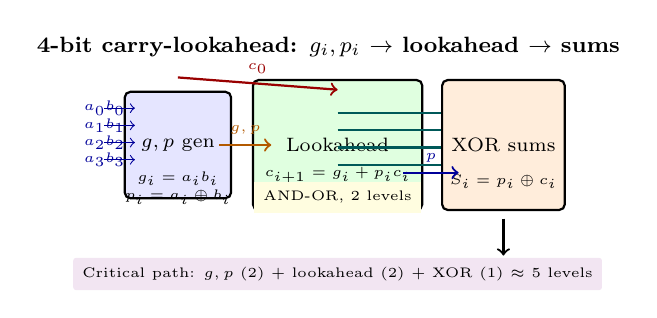
\begin{tikzpicture}[scale=0.78,every node/.style={font=\scriptsize}]
\node[font=\footnotesize\bfseries] at (3.8,3.15) {4-bit carry-lookahead: $g_i,p_i$ $\to$ lookahead $\to$ sums};
% g/p gen
\node[draw,thick,fill=blue!10,minimum width=1.35cm,minimum height=1.35cm,rounded corners=2pt] (gp) at (1.35,1.55) {$g,p$ gen};
\node[font=\tiny] at (1.35,1.0) {$g_i=a_i b_i$};
\node[font=\tiny] at (1.35,0.70) {$p_i=a_i\oplus b_i$};
\foreach \i in {0,1,2,3} \draw[->,thin,blue!60!black] (0.15,2.15-\i*0.28)--(0.65,2.15-\i*0.28) node[left,font=\tiny] {$a_{\i}b_{\i}$};
% Lookahead block
\node[draw,thick,fill=green!12,minimum width=2.15cm,minimum height=1.65cm,rounded corners=2pt] (la) at (3.95,1.55) {Lookahead};
\node[font=\tiny] at (3.95,1.05) {$c_{i+1}=g_i+p_i c_i$};
\node[font=\tiny,fill=yellow!12] at (3.95,0.70) {AND-OR, 2 levels};
\draw[->,thick,orange!70!black] (2.02,1.55)--(2.87,1.55) node[midway,above,font=\tiny] {$g,p$};
\draw[->,thick,red!60!black] (1.35,2.65)--(3.95,2.45) node[midway,above,font=\tiny] {$c_0$};
\foreach \i in {1,2,3,4} \draw[->,thick,teal!70!black] (3.95,2.35-\i*0.28)--(6.3,2.35-\i*0.28) node[right,font=\tiny] {$c_{\i}$};
% Sums
\node[draw,thick,fill=orange!14,minimum width=1.45cm,minimum height=1.65cm,rounded corners=2pt] (sum) at (6.65,1.55) {XOR sums};
\node[font=\tiny] at (6.65,0.95) {$S_i=p_i\oplus c_i$};
\draw[->,thick,blue!60!black] (5.02,1.10)--(5.92,1.10) node[midway,above,font=\tiny] {$p$};
\draw[->,thick] (6.65,0.35)--(6.65,-0.25) node[below,font=\tiny] {$S_3\dots S_0$};
\node[font=\tiny,fill=violet!10,rounded corners=1pt] at (3.95,-0.55) {Critical path: $g,p$ (2) + lookahead (2) + XOR (1) $\approx$ 5 levels};
\end{tikzpicture}
\caption{Carry-lookahead dataflow. All carries are computed in parallel from $g,p,c_0$ in two AND-OR levels, then XORed for sums.}
\label{fig:cla}
\end{figure}

\emph{Carry-select} trades off: compute two speculative results ($c_{\text{mid}}=0$ and $1$) for the upper half
and MUX-select when the real carry arrives---less logic than full CLA, faster than ripple.

\section{Subtraction and Overflow in Hardware}
Subtraction $A-B$ is $A+\bar B+1$ (two's complement negate: invert $B$ and set $c_0=1$). One adder does both
add and subtract with a $\mathit{SUB}$ control that XORs $B$ with $\mathit{SUB}$ and feeds $\mathit{SUB}$ as $c_0$.
Overflow $V = c_n\oplus c_{n-1}$ (carry into sign $\neq$ carry out) or equivalently, same-sign inputs producing opposite-sign sum.

\section{Multiplication}
\label{sec:multiplication}
Paper-and-pencil binary multiplication is shifts and adds. Two hardware styles:

\begin{itemize}
    \item \textbf{Array multiplier:} $n\times n$ grid of AND gates (partial products) plus adders summing rows---$O(n^2)$ gates, delay $O(n)$.
    \item \textbf{Shift-add (sequential):} one adder + shift register, iterating $n$ cycles---compact, used in microcode.
\end{itemize}
\emph{Booth recoding} handles signed two's complement directly by recoding runs of $1$s (e.g.\ $01110 = +16-2$),
reducing partial products and speeding signed multiply.

\begin{figure}[h]
\centering
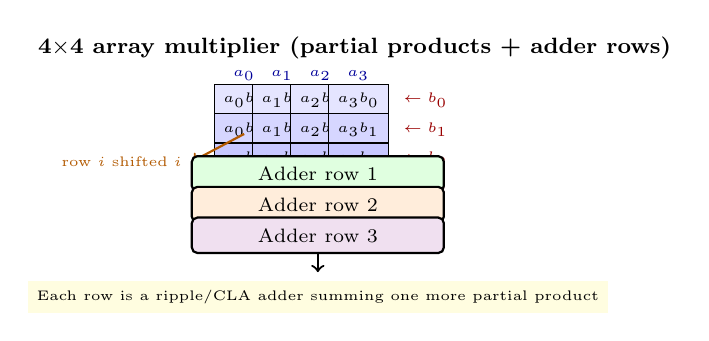
\begin{tikzpicture}[scale=0.78,every node/.style={font=\scriptsize}]
\node[font=\footnotesize\bfseries] at (2.8,3.0) {4$\times$4 array multiplier (partial products + adder rows)};
% Partial products grid
\foreach \i in {0,1,2,3} {
  \foreach \j in {0,1,2,3} {
    \pgfmathsetmacro{\x}{1.0+\j*0.62}
    \pgfmathsetmacro{\y}{2.15-\i*0.48}
    \node[draw,fill=blue!\the\numexpr 10+\i*6\relax,minimum width=0.50cm,minimum height=0.32cm,font=\tiny] at (\x,\y) {$a_{\j}b_{\i}$};
  }
  \node[font=\tiny,red!60!black] at (3.95,2.15-\i*0.48) {$\leftarrow b_{\i}$};
}
\foreach \j in {0,1,2,3} \node[font=\tiny,blue!60!black] at (1.0+\j*0.62,2.55) {$a_{\j}$};
% Shift illustration
\draw[->,thick,orange!70!black] (1.0,1.60)--(0.15,1.15) node[left,font=\tiny] {row $i$ shifted $i$};
% Adder rows
\node[draw,thick,fill=green!12,minimum width=3.2cm,minimum height=0.45cm,rounded corners=2pt] at (2.2,0.95) {Adder row 1};
\node[draw,thick,fill=orange!14,minimum width=3.2cm,minimum height=0.45cm,rounded corners=2pt] at (2.2,0.45) {Adder row 2};
\node[draw,thick,fill=violet!12,minimum width=3.2cm,minimum height=0.45cm,rounded corners=2pt] at (2.2,-0.05) {Adder row 3};
\draw[->,thick] (2.2,-0.32)--(2.2,-0.65) node[below,font=\tiny] {$P_7\dots P_0$ (8-bit product)};
\node[font=\tiny,fill=yellow!12] at (2.2,-1.05) {Each row is a ripple/CLA adder summing one more partial product};
\end{tikzpicture}
\caption{Array multiplier: each row of AND gates creates one partial product; successive adder rows accumulate them with increasing shift.}
\label{fig:array-mult}
\end{figure}

\section{Arithmetic Logic Unit (ALU)}
The ALU is a MUX of operations sharing one adder: inputs $A,B$, control $Op$ selects
arithmetic ($+,-,$ increment) or logic (AND, OR, XOR, NOT) plus shifts. Status flags:
\emph{C} carry out, \emph{Z} zero ($NOR$ of result), \emph{N} sign (MSB), \emph{V} signed overflow, used by branch logic.

\begin{figure}[h]
\centering
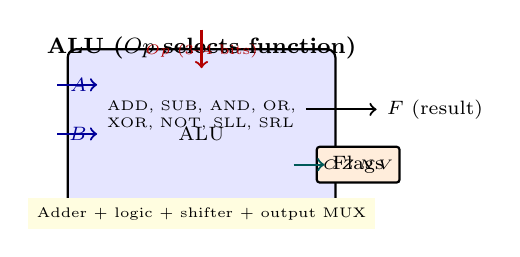
\begin{tikzpicture}[scale=0.78,every node/.style={font=\scriptsize}]
\node[draw,thick,fill=blue!10,minimum width=3.4cm,minimum height=2.15cm,rounded corners=3pt] (alu) at (2.5,0.75) {ALU};
\node[font=\footnotesize\bfseries] at (2.5,2.15) {ALU ($Op$ selects function)};
\draw[->,thick,blue!60!black] (0.15,1.55)--(0.80,1.55) node[left] {$A$};
\draw[->,thick,blue!60!black] (0.15,0.75)--(0.80,0.75) node[left] {$B$};
\draw[->,thick,red!70!black] (2.5,2.45)--(2.5,1.82) node[above,font=\tiny] {$Op$ (3--4 bits)};
\draw[->,thick] (4.20,1.15)--(5.35,1.15) node[right] {$F$ (result)};
% flags
\node[draw,thick,fill=orange!14,minimum width=1.05cm,minimum height=0.45cm,rounded corners=1pt] at (5.05,0.25) {Flags};
\node[font=\tiny] at (5.05,0.25) {$C\,Z\,N\,V$};
\draw[->,thick,teal!70!black] (4.00,0.25)--(4.50,0.25);
\node[font=\tiny,align=left] at (2.5,1.05) {ADD, SUB, AND, OR,\\XOR, NOT, SLL, SRL};
\node[font=\tiny,fill=yellow!12] at (2.5,-0.55) {Adder + logic + shifter + output MUX};
\end{tikzpicture}
\caption{ALU organization: one shared adder plus logic and shifter, multiplexed by the operation code; flags summarize the result for branching.}
\label{fig:alu}
\end{figure}


\section{Carry-Select, Prefix Adders, and Multiplication Tradeoffs}
\emph{Carry-select} partitions $n$ bits into blocks (e.g.\ $4+4+4+4$ for $n=16$), precomputes both $c_{in}=0$ and $1$ per block,
then MUX-selects. Delay $\approx$ block adder + $(n/{\rm blocksize}-1)$ MUX delays---between ripple and full CLA.
\emph{Parallel-prefix} (Kogge--Stone, Brent--Kung) generalises CLA to $O(\log n)$ depth with $O(n\log n)$ or $O(n)$ cost,
the standard choice for 32/64-bit ALU adders at GHz frequencies.

Multiplication area--time tradeoff: array is $O(n^2)$ gates but single-cycle; shift-add is $O(n)$ gates but $n$ cycles.
For $n=32$, Wallace/Dadda trees compress partial products with 3:2 counter arrays to $O(\log n)$ stages, used in high-performance multipliers.
\begin{example}[Flag generation]
Result $R=A+B$: $C=$ carry out, $Z=\bigwedge_i \bar R_i$ (NOR), $N=R_{n-1}$, $V=C_n\oplus C_{n-1}$.
Branch conditions combine them: e.g.\ signed $A<B$ iff $N\oplus V=1$ for two's complement.
\end{example}

% ============================================================

% ============================================================
\section{Chapter Notes}
CLA was described by Weinberger and Smith (1958); Booth's algorithm (1951) sped early computer multipliers.
Modern ALUs use parallel-prefix adders (Kogge--Stone, Brent--Kung) that generalise CLA to $O(\log n)$ delay.

% ============================================================
\section{Division Preview and Fixed-Point Scaling}
Division is the hardest basic operation---iterative subtract-and-shift (restoring or non-restoring) takes $n$ cycles for $n$ bits,
with careful handling of two's complement signs. We omit full design here (computer arithmetic course), but note that multiplication
and division by $2^k$ are just shifts, and fixed-point scaling (e.g.\ Q15 format: 1 sign + 15 fractional bits) uses this to implement
fractional arithmetic with integer hardware, ubiquitous in DSP and embedded control.

% ============================================================

\paragraph{Signed overflow vs.\ carry.} Carry $C$ is unsigned overflow; $V$ is signed overflow. For addition,
$V = (A_{n-1}\!\oplus\!R_{n-1})\cdot(B_{n-1}\!\oplus\!R_{n-1})$ or $C_n\!\oplus\!C_{n-1}$. Hardware computes both
in parallel from the adder's internal carries. Branch logic selects which flag to test based on signed vs.\ unsigned
interpretation of the preceding operation (e.g.\ \texttt{BCC} vs.\ \texttt{BVS} in 6502/ARM).

\paragraph{Shifter and rotator.} A \emph{barrel shifter} rotates or shifts $n$ bits by any amount in $O(\log n)$ MUX stages
(e.g.\ 32-bit shift in 5 stages of 2:1 MUXes controlled by shift-amount bits). Shifts are essential for normalization in
floating-point and for alignment in addition. Rotates preserve bits (useful in cryptography); arithmetic right shift replicates
the sign bit to preserve two's complement value.

\paragraph{Multiplication correctness sketch.} Array multiplier sums partial products $a_jb_i$ at column $j+i$; each adder row preserves
$\sum$ partials = product. By induction on rows, after $k$ rows the partial sum equals $\sum_{i<k}\sum_j a_jb_i2^{j+i}$,
and after $n$ rows the full $2n$-bit product. Booth's recoding maintains the same invariant with fewer non-zero partials.

\paragraph{Cost vs.\ delay summary.} Ripple: $O(n)$ gates, $O(n)$ delay. CLA: $O(n^2)$ (na\"ive) or $O(n)$ with grouping, $O(\log n)$ delay. Carry-select: $\approx1.5\times$ ripple gates, $\approx O(\sqrt n)$ delay. Choose by constraints: area-limited $\to$ ripple/carry-select, speed-limited $\to$ prefix CLA.

\section{Exercises}
\label{sec:ch07-exercises}
\begin{enumerate}[label=E7.\arabic*, leftmargin=*, itemsep=0.8em]
    \item \textbf{CLA equations.} For $n=4$, write $c_1\dots c_4$ in terms of $g_i,p_i,c_0$. Group as 4-bit block with $G=g_3+p_3g_2+p_3p_2g_1+p_3p_2p_1g_0$, $P=p_3p_2p_1p_0$.
    \item \textbf{Delay.} Ripple $n=16$ with $t_{FA}=2$ vs.\ CLA with $t_{gp}=2$, $t_{look}=2$, $t_{xor}=1$. Compute worst-case delays and speedup.
    \item \textbf{Subtractor.} Show how one adder with $SUB$ control computes both $A+B$ and $A-B$. Where does overflow $V$ come from? Test $A=0111$, $B=0001$.
    \item \textbf{Booth.} Multiply $6\times(-3)$ ($0101\times1101$ in 4-bit two's complement) using Booth recoding. List partial products and final product.
    \item \textbf{ALU flags.} For $A=1011$, $B=0101$, compute $A+B$, $A-B$, $A\;\&\;B$ in 4-bit two's complement and give $C,Z,N,V$ for each.
\end{enumerate}
% End of Chapter 7
